%mainfile: rapport.tex


\section{Structures de données}
\label{section:storage}

\subsection{Le modèle - vue d'ensemble}

Le modèle des structures de données utilisées par PIE est basé autour de la notion de
flux, à ce flux est associé un état. Ces flux sont caractérisés par un couple d'informations
garantissant leur unicité. Il s'agit de la provenance du flux - le champ FROM du protocole
(\cfsection{mesg}) - et de l'identité de l'utilisateur associé a ce flux - le champs NICK
du protocole (\cfsection{mesg}).\\

En plus de celles précitées, un flux est un objet constitué d'un ensemble de caractéristiques.
Ces caractéristiques sont d'une part les informations liées à la notion d'identité de utilisateur
associé au flux, de l'autre celles liées - au même titre que l'état - à sa gestion. \\

Les informations caractérisant un utilisateur associé à un flux ne sont pas - par défaut -
transmises par celui-ci (à l'exception du couple NICK/FROM). Lorsque 
l'utilisateur local de PIE en fait la demande, une requête unidirectionnelle (de type \textbf{getinfo})
peut alors être adressée au flux en question; si une réponse de sa part est reçu alors
les informations le concernant sont mises à jour. \\

Du fait de leur unicité, les flux constituent un ensemble, une collection d'objets uniques (\cfsection{vin}).
L'état définit une relation entre un flux et l'utilisateur local de l'application. Un flux
peut être : \\

\begin{itemize}
	\item \textbf{available}, l'utilisateur local a accès à ce flux,
    \item \textbf{forwarded}, l'utilisateur local transmet le flux à des paires,
    \item \textbf{subscribed}, l'utilisateur local est abonné au flux. \\
\end{itemize}

Ces états possibles se superposent, car un flux peut avoir les trois états simultanément.
L'état d'un flux est une caractéristique offrant les relations ensemblistes suivantes : \\

\begin{itemize}
	\item quelque soit un flux x alors il appartient à \textbf{available},
	\item \textbf{subscribed} est un sous ensemble d'\textbf{available},
	\item \textbf{forwarded} est un sous ensemble d'\textbf{available},
	\item \textbf{subscribed} U \textbf{forwarded} est inclus ou égale à \textbf{available},
	\item L'intersection de \textbf{subscribed} et \textbf{forwarded} est éventuellement non vide.\\
\end{itemize}

L'état d'un flux est une caractéristique de gestion, cette caractéristique est modélisée
par l'utilisation de trois listes : \\

\begin{itemize}
	\item la liste des flux \textbf{available}, soit l'ensemble des flux,
	\item la liste des flux \textbf{forwarded}, le sous-ensemble des flux transmis,
	\item la liste des flux \textbf{subscribed}, le sous-ensemble des flux auquel l'utilisateur local est abonné. \\
\end{itemize}

Un gestion unifiée de ces structures de données est offerte par un sous-système de PIE,
l'interface de stockage. Cette interface permet la manipulation des flux, des informations 
qui leur sont associées et de leurs états, c'est l'interface de plus haut niveau pour la
manipulation des flux. L'interface de stockage est une interface de gestion, automatisant
les différentes taches inhérentes à cette gestion, elle met à profit les relations ensemblistes 
exposées à travers l'utilisation de listes. \\

Le schéma suivant présente les structures de données précitées et les relations (logiques)
entre chacunes :  \\

\begin{center}
    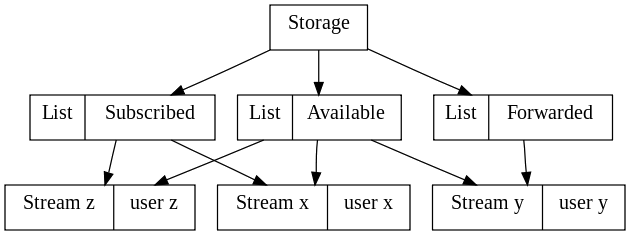
\includegraphics[width=0.8\textwidth]{img/struct.png}
\end{center}

\subsection{Implémentation}

Le modèle présenté dans le précèdent paragraphe a conduit à l'implémentation
présentée maintenant. Chacun des objets considérés dans le modèle dispose d'une
interface qui lui est propre. Il y a donc quatre interfaces de gestion différentes : \\

\begin{itemize}
	\item \textbf{user} : interface de gestion des utilisateurs associés aux flux,
	\item \textbf{stream} : interface de gestion des flux,
	\item \textbf{list}:  interface de gestion des listes de flux,
	\item \textbf{storage} : l'interface de stockage, plus haut niveau d'abstraction. \\
\end{itemize}


Chacune des interfaces précitées offre une couche d'abstraction permettant la manipulation
des objets qu'elle modélise. Elles sont définies par deux niveaux : Il y a d'une part, des
fonctions de manipulation globales des objets fournis par l'interface (telle que seraient
des fonctions statiques d'une classe en java) et de l'autre ,des fonctions de manipulation
des objets par eux mêmes (le pendant des méthodes en java). Les fonctions et méthodes des
différentes interfaces permettent par exemple la recherche d'objets en fonction de la valeur
de leur attributs autant que leur mise à jour ou encore leur destruction.

\subsubsection{Interface User}

Un utilisateur (\textbf{user}) est représenté par un objet disposant
d'un certain nombre de caractéristiques, celles ci sont : \\

\begin{itemize}
	\item \textbf{id} : information de gestion initialisée à la création,
	\item \textbf{nickname}	: correspond au champ \textbf{NICK} définit dans le protocol,
	\item \textbf{email} : l'adresse email de l'utilisateur (optionnelle),
	\item \textbf{fullname} : son nom (optionnelle),
	\item \textbf{firstname} : son prénom (optionnelle),
	\item \textbf{phone\_nb} : son numéro de téléphone (optionnelle),
	\item \textbf{age} : son age (optionnelle),
	\item \textbf{sex} : son sexe (optionnelle),
	\item \textbf{dest} : sa destination actuelle (optionnelle),
	\item \textbf{desc} : se description de l'utilisateur (optionnelle).\\
\end{itemize}

Les caractéristiques notées optionnelles sont celles n'ayant pas d'impact
sur le fonctionnement de PIE en interne, elles n'ont pour objet que d'offrir
un profil plus détaillé (informations obtenues par une requête \textbf{getinfo}).
 
\subsubsection{Interface Stream}

Ces objets utilisateur, sont implémentés en utilisant le package Itcl qui offre
une couche abstraction de type objet au langage TCL, ils sont contenus
(associés) dans un object de type flux (\textbf{stream}). L'objet \textbf{stream}
est defini par les champs : \\

\begin{itemize}
	\item \textbf{stream\_id} : information de gestion initialisée à la création,
	\item \textbf{car\_id} : information correspondant au champ FROM du protocol,
	\item \textbf{time\_available} : l'heure locale depuis laquelle le flux est disponible,
	\item \textbf{time\_lastmsg} : l'heure locale du dernier message reçu de ce flux,
	\item \textbf{time\_lasthello} : l'heure locale du dernier message de type hello,
	\item \textbf{nb\_mesg} : le nombre de messages envoyés par ce flux,
	\item \textbf{user} : l'objet utilisateur présenté dans le précédent paragraphe,
	\item un certain nombre d'informations de gestion pour le protocole.
\end{itemize}

\subsubsection{Interface List}

Les listes bien que nativement présentent dans le langage TCL bénéficient également
d'une interface particulière et écrite par nos soins. Cette interface permet une gestion
cohérente au modèle ensembliste - unicité des éléments dans chaque liste.

\subsubsection{Interface Storage}

Enfin l'interface de stockage est celle permettant la gestion de l'ensemble, c'est 
celle présentant le plus haut niveau d'abstraction, c'est donc à travers cette interface
que sont manipulés tous les objets du modèle. Le stockage maintient 4 listes :\\

\begin{itemize}
	\item la liste des flux \textbf{available}, soit l'ensemble des flux,
	\item la liste des flux \textbf{forwarded}, sous-ensemble des flux transmis,
	\item la liste des flux \textbf{subscribed}, sous-ensemble des flux souscrits localement,
	\item la liste des flux \textbf{forgotten}, les flux devenus indisponible. \\
\end{itemize}

Lorsque un nouveau flux est crée, cela correspond à la réception d'informations de sa part, l'objet
associé à ce flux est alors initialisé. Il est crée à travers l'interface de stockage des flux et
bénéficie de l'état disponible (\textbf{available}). Si l'utilisateur décide de s'y abonner, alors
le flux bénéficie également de cet état et à ce titre, est mis dans la liste associée (\textbf{subscribed}).
Enfin un flux pour lequel PIE est informé qu'il intéresse un pair, sera mis dans la liste des flux
transmis (\textbf{forwarded}). \\

Lorsqu'un flux devient indisponible, plutôt que de détruire l'objet associé, celui-ci est placé dans la
liste \textbf{forgotten}, il tombe dans les limbes. Il s'agit d'une optimisation et d'un écart au modèle
présenté : ne pas détruire ce flux permet de le rendre disponible de nouveau à l'utilisateur local et
cela sans sur-coup au niveau des ressources locales. De plus, si d'aventure, des informations avaient
au préalable été obtenues sur l'utilisateur associé au dit flux (via une requête de type getinfo) alors
il n'est pas nécessaire de les redemander ensuite, ce qui évite de saturer le média de communication. \\

L'évolution des états d'un flux peut être repésenté par le schéma suivant :

\begin{center}
    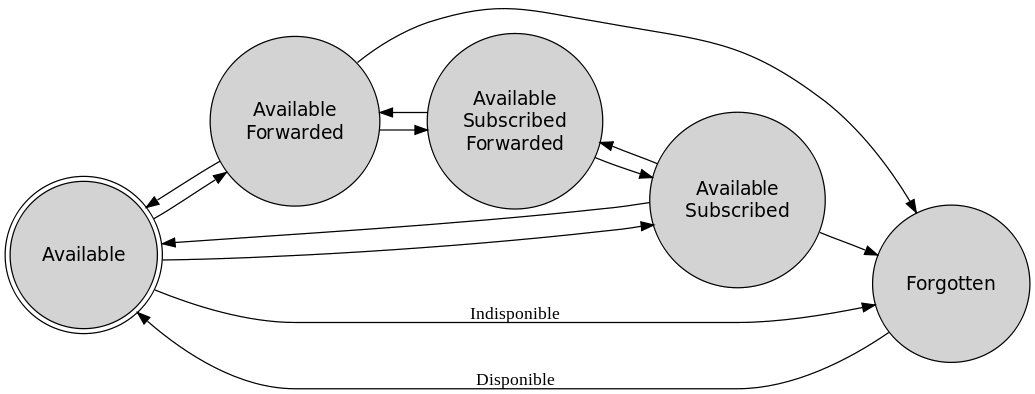
\includegraphics[width=1\textwidth]{img/state.png}
\end{center}

Les listes ne contiennent en fait que des références vers les objets. C'est à l'interface de
stockage de garantir les propriétés précédemment exposées. \\

